% =========================================================
% Chapter 5 - Database Design
% Project: AITasker
%
% Yêu cầu trong main.tex:
% \usepackage{graphicx}
% \usepackage{float}
% \usepackage{longtable}
% \usepackage{array}
% \graphicspath{{figures/}}
%
% Tên hình đúng trong thư mục figures:
%   ERD.png
%   Class.png
% =========================================================

\chapter{Thiết kế cơ sở dữ liệu}
\label{chap:database}

\section{Giới thiệu}
\label{sec:database-introduction}

Chương này trình bày thiết kế cơ sở dữ liệu của hệ thống AITasker. Nội dung bao gồm mô hình dữ liệu mức khái niệm thông qua Entity Relationship Diagram (ERD), mô hình lớp thông qua Class Diagram, mô tả các thực thể chính, quan hệ giữa các bảng, các ràng buộc toàn vẹn và từ điển dữ liệu.

Hệ thống sử dụng PostgreSQL làm hệ quản trị cơ sở dữ liệu và SQLAlchemy ORM để ánh xạ giữa các đối tượng trong ứng dụng với các bảng dữ liệu.

\section{Mục tiêu thiết kế}
\label{sec:database-objectives}

Thiết kế cơ sở dữ liệu hướng tới các mục tiêu:

\begin{itemize}
    \item Đảm bảo tính nhất quán dữ liệu.
    \item Giảm dư thừa thông tin.
    \item Hỗ trợ truy vấn hiệu quả.
    \item Đảm bảo toàn vẹn tham chiếu.
    \item Dễ bảo trì và mở rộng.
    \item Phù hợp với kiến trúc FastAPI và SQLAlchemy.
\end{itemize}

\section{Entity Relationship Diagram}
\label{sec:erd}

\begin{figure}[H]
    \centering
    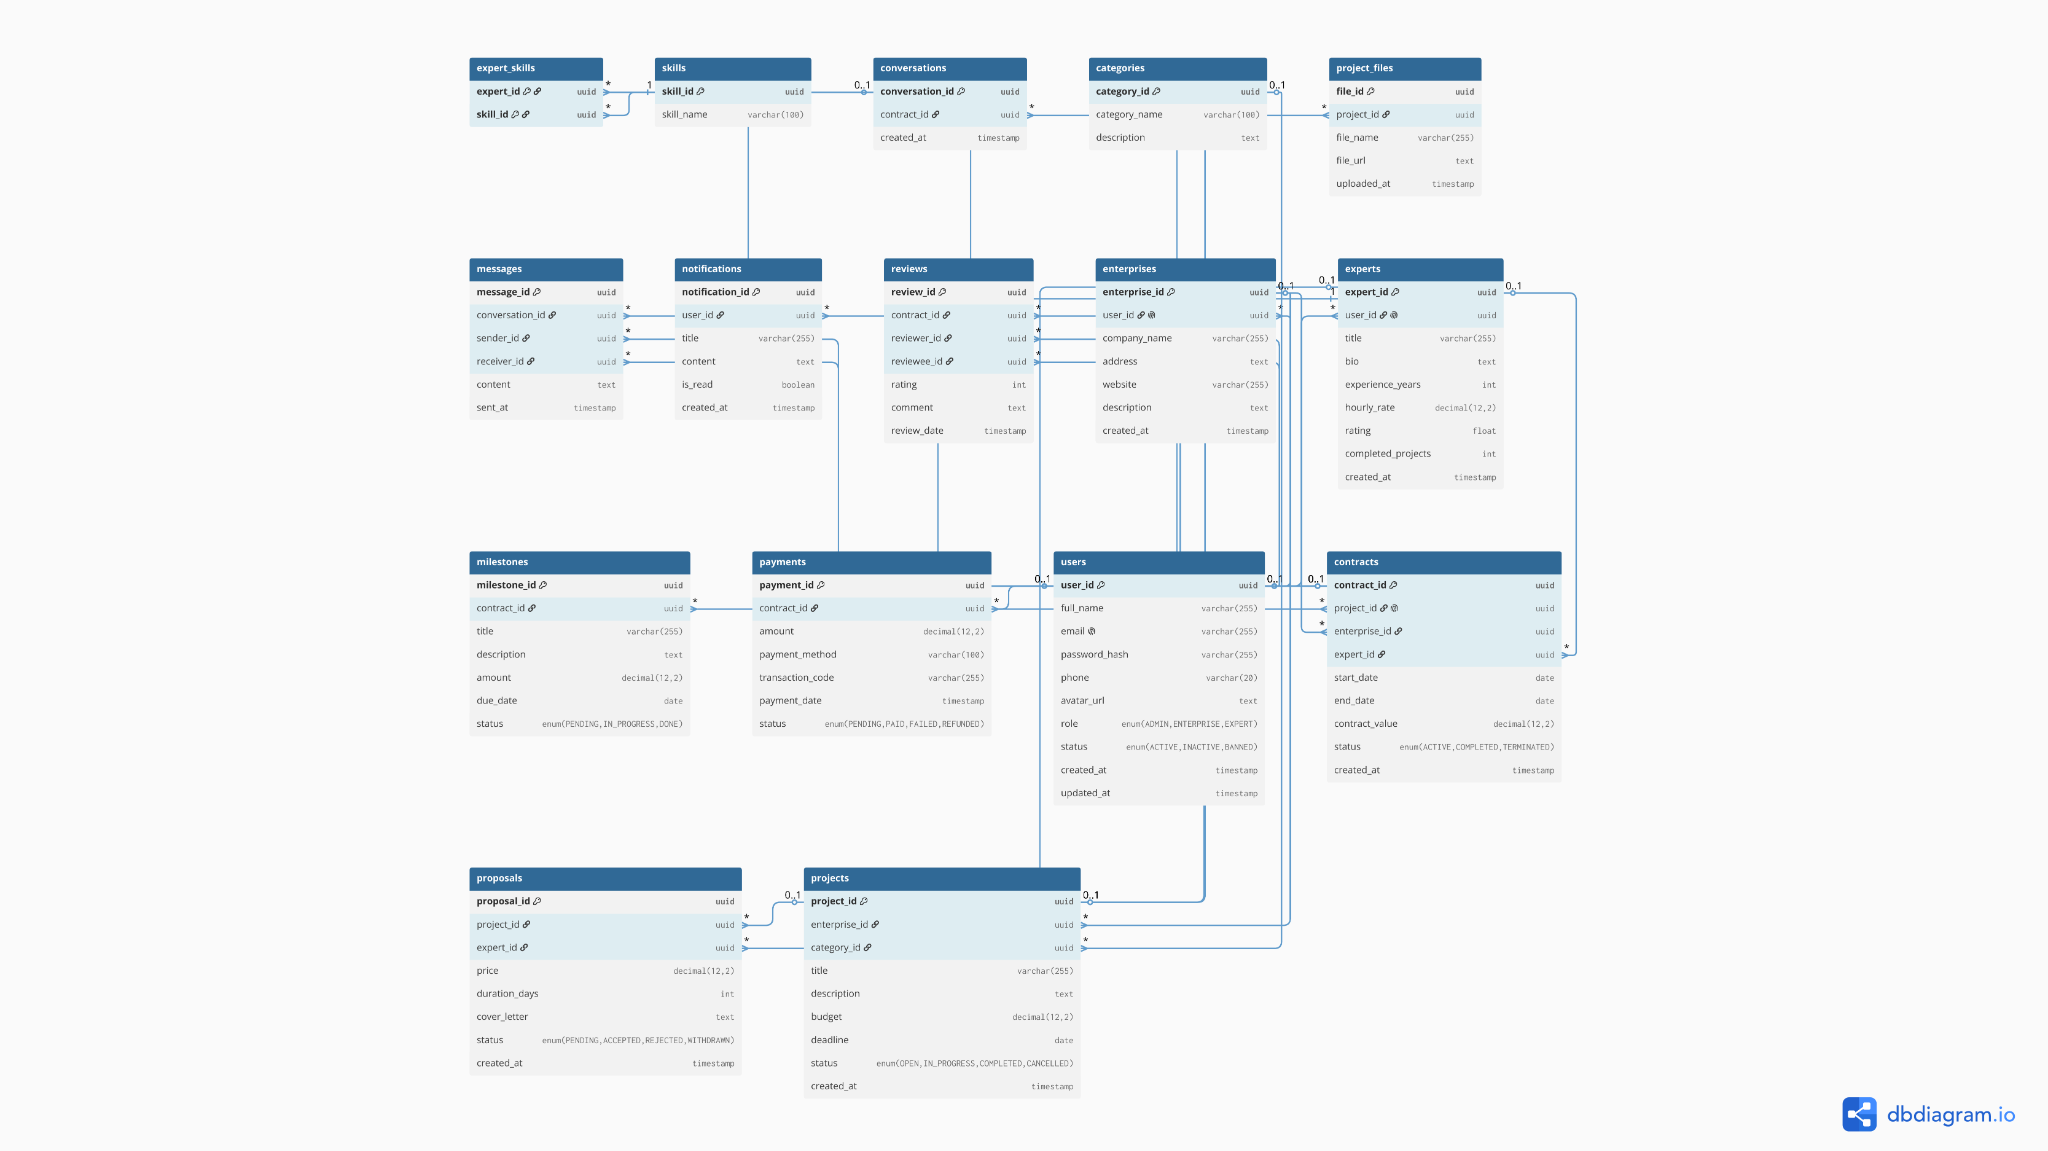
\includegraphics[width=\textwidth]{ERD.png}
    \caption{Entity Relationship Diagram của AITasker}
    \label{fig:erd}
\end{figure}

ERD mô tả các thực thể chính của hệ thống và quan hệ giữa chúng. Các thực thể bao gồm người dùng, doanh nghiệp, chuyên gia, dự án, đề xuất, hợp đồng, milestone, thanh toán, đánh giá, kỹ năng, hội thoại, tin nhắn và thông báo.

\section{Class Diagram}
\label{sec:class-diagram}

\begin{figure}[H]
    \centering
    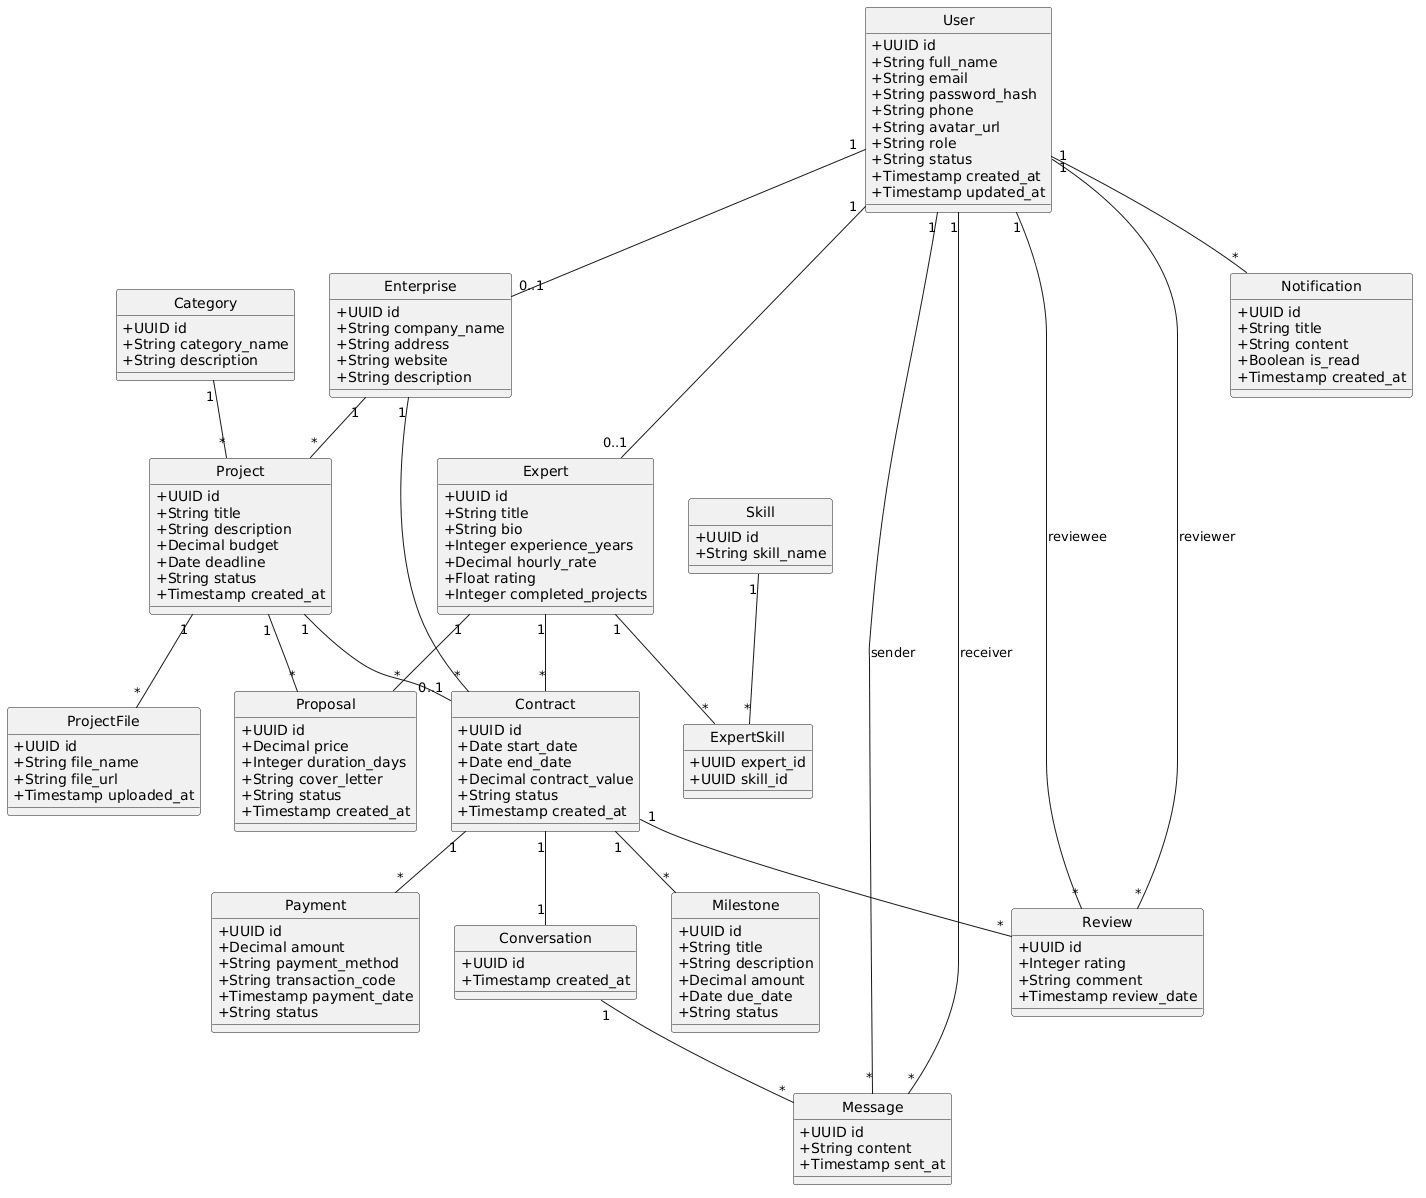
\includegraphics[width=\textwidth]{Class.png}
    \caption{Class Diagram của AITasker}
    \label{fig:class}
\end{figure}

Class Diagram mô tả các lớp trong hệ thống, thuộc tính của từng lớp và quan hệ giữa các lớp. Mô hình này hỗ trợ việc ánh xạ sang các model SQLAlchemy ở tầng backend.

\section{Các thực thể chính}
\label{sec:main-entities}

\subsection{User}

Thực thể User lưu thông tin xác thực và phân quyền người dùng.

\begin{itemize}
    \item \texttt{id}
    \item \texttt{full\_name}
    \item \texttt{email}
    \item \texttt{password\_hash}
    \item \texttt{phone}
    \item \texttt{avatar\_url}
    \item \texttt{role}
    \item \texttt{status}
    \item \texttt{created\_at}
    \item \texttt{updated\_at}
\end{itemize}

Quan hệ:

\begin{itemize}
    \item Một User có thể liên kết với một Enterprise hoặc một Expert.
    \item Một User có nhiều Notification.
    \item Một User có thể gửi và nhận nhiều Message.
    \item Một User có thể tạo hoặc nhận Review.
\end{itemize}

\subsection{Enterprise}

Thực thể Enterprise lưu thông tin doanh nghiệp.

\begin{itemize}
    \item \texttt{id}
    \item \texttt{user\_id}
    \item \texttt{company\_name}
    \item \texttt{address}
    \item \texttt{website}
    \item \texttt{description}
    \item \texttt{created\_at}
\end{itemize}

Quan hệ:

\begin{itemize}
    \item Một Enterprise thuộc một User.
    \item Một Enterprise có nhiều Project.
    \item Một Enterprise có thể tham gia nhiều Contract.
\end{itemize}

\subsection{Expert}

Thực thể Expert lưu hồ sơ chuyên gia AI.

\begin{itemize}
    \item \texttt{id}
    \item \texttt{user\_id}
    \item \texttt{title}
    \item \texttt{bio}
    \item \texttt{experience\_years}
    \item \texttt{hourly\_rate}
    \item \texttt{rating}
    \item \texttt{completed\_projects}
    \item \texttt{created\_at}
\end{itemize}

Quan hệ:

\begin{itemize}
    \item Một Expert thuộc một User.
    \item Một Expert có nhiều Skill thông qua ExpertSkill.
    \item Một Expert có nhiều Proposal.
    \item Một Expert tham gia nhiều Contract.
\end{itemize}

\subsection{Category}

Thực thể Category dùng để phân loại dự án.

\begin{itemize}
    \item \texttt{id}
    \item \texttt{category\_name}
    \item \texttt{description}
\end{itemize}

Quan hệ:

\begin{itemize}
    \item Một Category có nhiều Project.
\end{itemize}

\subsection{Project}

Thực thể Project lưu thông tin dự án AI.

\begin{itemize}
    \item \texttt{id}
    \item \texttt{enterprise\_id}
    \item \texttt{category\_id}
    \item \texttt{title}
    \item \texttt{description}
    \item \texttt{budget}
    \item \texttt{deadline}
    \item \texttt{status}
    \item \texttt{created\_at}
\end{itemize}

Quan hệ:

\begin{itemize}
    \item Một Project thuộc một Enterprise.
    \item Một Project thuộc một Category.
    \item Một Project có nhiều Proposal.
    \item Một Project có nhiều ProjectFile.
    \item Một Project có tối đa một Contract đang hoạt động.
\end{itemize}

\subsection{ProjectFile}

Thực thể ProjectFile lưu thông tin tệp đính kèm của dự án.

\begin{itemize}
    \item \texttt{id}
    \item \texttt{project\_id}
    \item \texttt{file\_name}
    \item \texttt{file\_url}
    \item \texttt{uploaded\_at}
\end{itemize}

\subsection{Proposal}

Thực thể Proposal lưu đề xuất của chuyên gia.

\begin{itemize}
    \item \texttt{id}
    \item \texttt{project\_id}
    \item \texttt{expert\_id}
    \item \texttt{price}
    \item \texttt{duration\_days}
    \item \texttt{cover\_letter}
    \item \texttt{status}
    \item \texttt{created\_at}
\end{itemize}

Các trạng thái chính:

\begin{itemize}
    \item \texttt{PENDING}
    \item \texttt{ACCEPTED}
    \item \texttt{REJECTED}
    \item \texttt{WITHDRAWN}
\end{itemize}

\subsection{Contract}

Thực thể Contract được tạo khi một proposal được chấp nhận.

\begin{itemize}
    \item \texttt{id}
    \item \texttt{project\_id}
    \item \texttt{enterprise\_id}
    \item \texttt{expert\_id}
    \item \texttt{start\_date}
    \item \texttt{end\_date}
    \item \texttt{contract\_value}
    \item \texttt{status}
    \item \texttt{created\_at}
\end{itemize}

Quan hệ:

\begin{itemize}
    \item Một Contract thuộc một Project.
    \item Một Contract liên kết một Enterprise và một Expert.
    \item Một Contract có nhiều Milestone.
    \item Một Contract có nhiều Payment.
    \item Một Contract có một Conversation.
    \item Một Contract có nhiều Review.
\end{itemize}

\subsection{Milestone}

Thực thể Milestone lưu từng giai đoạn của hợp đồng.

\begin{itemize}
    \item \texttt{id}
    \item \texttt{contract\_id}
    \item \texttt{title}
    \item \texttt{description}
    \item \texttt{amount}
    \item \texttt{due\_date}
    \item \texttt{status}
\end{itemize}

Các trạng thái chính:

\begin{itemize}
    \item \texttt{PENDING}
    \item \texttt{IN\_PROGRESS}
    \item \texttt{DONE}
    \item \texttt{CANCELLED}
\end{itemize}

\subsection{Payment}

Thực thể Payment lưu thông tin giao dịch.

\begin{itemize}
    \item \texttt{id}
    \item \texttt{contract\_id}
    \item \texttt{amount}
    \item \texttt{payment\_method}
    \item \texttt{transaction\_code}
    \item \texttt{payment\_date}
    \item \texttt{status}
\end{itemize}

Các trạng thái chính:

\begin{itemize}
    \item \texttt{PENDING}
    \item \texttt{PAID}
    \item \texttt{FAILED}
    \item \texttt{REFUNDED}
\end{itemize}

\subsection{Conversation}

Thực thể Conversation đại diện cho một hội thoại liên quan đến hợp đồng.

\begin{itemize}
    \item \texttt{id}
    \item \texttt{contract\_id}
    \item \texttt{created\_at}
\end{itemize}

Quan hệ:

\begin{itemize}
    \item Một Conversation thuộc một Contract.
    \item Một Conversation có nhiều Message.
\end{itemize}

\subsection{Message}

Thực thể Message lưu nội dung trao đổi giữa người dùng.

\begin{itemize}
    \item \texttt{id}
    \item \texttt{conversation\_id}
    \item \texttt{sender\_id}
    \item \texttt{receiver\_id}
    \item \texttt{content}
    \item \texttt{sent\_at}
\end{itemize}

\subsection{Review}

Thực thể Review lưu điểm đánh giá và nhận xét sau khi hoàn thành hợp đồng.

\begin{itemize}
    \item \texttt{id}
    \item \texttt{contract\_id}
    \item \texttt{reviewer\_id}
    \item \texttt{reviewee\_id}
    \item \texttt{rating}
    \item \texttt{comment}
    \item \texttt{review\_date}
\end{itemize}

\subsection{Notification}

Thực thể Notification lưu thông báo gửi đến người dùng.

\begin{itemize}
    \item \texttt{id}
    \item \texttt{user\_id}
    \item \texttt{title}
    \item \texttt{content}
    \item \texttt{is\_read}
    \item \texttt{created\_at}
\end{itemize}

\subsection{Skill và ExpertSkill}

Skill lưu danh mục kỹ năng chuyên môn.

\begin{itemize}
    \item \texttt{id}
    \item \texttt{skill\_name}
\end{itemize}

ExpertSkill là bảng trung gian cho quan hệ nhiều--nhiều giữa Expert và Skill.

\begin{itemize}
    \item \texttt{expert\_id}
    \item \texttt{skill\_id}
\end{itemize}

\section{Quan hệ giữa các bảng}
\label{sec:table-relationships}

\begin{table}[H]
    \centering
    \caption{Các quan hệ chính giữa các bảng}
    \label{tab:table-relationships}
    \begin{tabular}{|p{4.1cm}|p{2.8cm}|p{6.8cm}|}
        \hline
        \textbf{Bảng nguồn} & \textbf{Quan hệ} & \textbf{Bảng đích} \\ \hline
        User & 1:0..1 & Enterprise \\ \hline
        User & 1:0..1 & Expert \\ \hline
        Enterprise & 1:N & Project \\ \hline
        Category & 1:N & Project \\ \hline
        Project & 1:N & ProjectFile \\ \hline
        Project & 1:N & Proposal \\ \hline
        Expert & 1:N & Proposal \\ \hline
        Project & 1:0..1 & Contract \\ \hline
        Contract & 1:N & Milestone \\ \hline
        Contract & 1:N & Payment \\ \hline
        Contract & 1:1 & Conversation \\ \hline
        Conversation & 1:N & Message \\ \hline
        Contract & 1:N & Review \\ \hline
        Expert & N:M & Skill \\ \hline
        User & 1:N & Notification \\ \hline
    \end{tabular}
\end{table}

\section{Từ điển dữ liệu}
\label{sec:data-dictionary}

\begin{longtable}{|p{3.0cm}|p{3.0cm}|p{2.2cm}|p{5.4cm}|}
\caption{Từ điển dữ liệu rút gọn}
\label{tab:data-dictionary} \\ \hline
\textbf{Bảng} & \textbf{Trường} & \textbf{Kiểu} & \textbf{Ý nghĩa} \\ \hline
\endfirsthead
\hline
\textbf{Bảng} & \textbf{Trường} & \textbf{Kiểu} & \textbf{Ý nghĩa} \\ \hline
\endhead

users & \texttt{id} & UUID & Định danh người dùng. \\ \hline
users & \texttt{email} & VARCHAR & Email đăng nhập, duy nhất. \\ \hline
users & \texttt{password\_hash} & VARCHAR & Mật khẩu đã được băm. \\ \hline
projects & \texttt{id} & UUID & Định danh dự án. \\ \hline
projects & \texttt{enterprise\_id} & UUID/FK & Doanh nghiệp sở hữu dự án. \\ \hline
projects & \texttt{category\_id} & UUID/FK & Danh mục của dự án. \\ \hline
proposals & \texttt{project\_id} & UUID/FK & Dự án nhận đề xuất. \\ \hline
proposals & \texttt{expert\_id} & UUID/FK & Chuyên gia gửi đề xuất. \\ \hline
contracts & \texttt{project\_id} & UUID/FK & Dự án được ký hợp đồng. \\ \hline
contracts & \texttt{expert\_id} & UUID/FK & Chuyên gia thực hiện hợp đồng. \\ \hline
milestones & \texttt{contract\_id} & UUID/FK & Hợp đồng chứa milestone. \\ \hline
payments & \texttt{contract\_id} & UUID/FK & Hợp đồng liên quan đến thanh toán. \\ \hline
reviews & \texttt{contract\_id} & UUID/FK & Hợp đồng được đánh giá. \\ \hline
notifications & \texttt{user\_id} & UUID/FK & Người dùng nhận thông báo. \\ \hline
messages & \texttt{conversation\_id} & UUID/FK & Hội thoại chứa tin nhắn. \\ \hline
\end{longtable}

\section{Các ràng buộc toàn vẹn}
\label{sec:integrity-constraints}

\begin{itemize}
    \item Email người dùng là duy nhất.
    \item Proposal phải tham chiếu đến Project và Expert hợp lệ.
    \item Mỗi Expert chỉ được gửi một Proposal cho một Project.
    \item Contract chỉ được tạo khi Proposal được chấp nhận.
    \item Một Project chỉ có tối đa một Contract đang hoạt động.
    \item Milestone phải thuộc một Contract hợp lệ.
    \item Payment chỉ được tạo cho Contract hoặc Milestone hợp lệ.
    \item Review chỉ được tạo sau khi Contract hoàn thành.
    \item Rating phải nằm trong khoảng từ 1 đến 5.
    \item Tất cả khóa ngoại phải đảm bảo toàn vẹn tham chiếu.
\end{itemize}

\section{Chuẩn hóa dữ liệu}
\label{sec:normalization}

Cơ sở dữ liệu được thiết kế hướng tới chuẩn hóa bậc ba (3NF).

\begin{itemize}
    \item Mỗi thuộc tính chứa một giá trị nguyên tử.
    \item Không tồn tại nhóm lặp trong một bảng.
    \item Các thuộc tính không khóa phụ thuộc đầy đủ vào khóa chính.
    \item Hạn chế phụ thuộc bắc cầu không cần thiết.
    \item Quan hệ nhiều--nhiều được tách thành bảng trung gian.
\end{itemize}

\section{Chỉ mục và hiệu năng truy vấn}
\label{sec:index-strategy}

Các cột nên được tạo chỉ mục gồm:

\begin{itemize}
    \item \texttt{users.email}
    \item Các khóa ngoại như \texttt{project\_id}, \texttt{expert\_id}, \texttt{contract\_id}.
    \item Các trường trạng thái thường dùng để lọc.
    \item Các trường thời gian thường dùng để sắp xếp.
\end{itemize}

Việc sử dụng chỉ mục giúp cải thiện tốc độ tìm kiếm dự án, proposal, hợp đồng và thông báo.

\section{Sao lưu và phục hồi}
\label{sec:backup-recovery}

Hệ thống cần hỗ trợ:

\begin{itemize}
    \item Sao lưu PostgreSQL định kỳ.
    \item Lưu bản sao backup ở vị trí an toàn.
    \item Kiểm tra khả năng phục hồi dữ liệu.
    \item Theo dõi lỗi transaction và lỗi kết nối.
    \item Không lưu khóa bí mật hoặc mật khẩu trong dữ liệu backup không được bảo vệ.
\end{itemize}

\section{Kết luận}
\label{sec:database-conclusion}

Thiết kế cơ sở dữ liệu của AITasker đáp ứng yêu cầu lưu trữ và quản lý toàn bộ vòng đời dự án AI. Mô hình dữ liệu hỗ trợ các nghiệp vụ từ quản lý người dùng, dự án, proposal, hợp đồng, milestone, thanh toán, nhắn tin đến đánh giá và thông báo.

Việc sử dụng PostgreSQL kết hợp SQLAlchemy ORM giúp đảm bảo tính nhất quán, dễ bảo trì và thuận tiện khi mở rộng hệ thống trong tương lai.
